% ICLR 2026 Paper Template — 中文逐句对应版
% 与 main.tex 同构：同一批图表 PDF、同一 RECOMPUTED_MACROS 数字宏；
% 仅正文与图表 caption 译为中文，图内英文标签保留原始实验命名。
% 编译：latexmk -xelatex main-zh.tex

\PassOptionsToPackage{table}{xcolor}
\documentclass{article}
\usepackage{iclr2027_conference,times}

% Math
\usepackage{amsmath,amssymb,amsfonts,amsthm,mathtools}

% Typography
\usepackage[utf8]{inputenc}
\usepackage[T1]{fontenc}
\usepackage{hyperref}
\usepackage{url}
\usepackage{booktabs}
\usepackage{array}
\usepackage{microtype}
\usepackage{xcolor}
\usepackage{graphicx}
\usepackage{subcaption}
\usepackage{multirow}
\usepackage{algorithm}
\usepackage{algorithmic}

% 中文（xelatex + Fandol 字体集）
\usepackage[UTF8]{ctex}

% cleveref must be loaded AFTER hyperref
\usepackage[capitalize,noabbrev]{cleveref}
\hypersetup{hidelinks}

% Theorems（环境名中文化，编号规则同英文版）
\theoremstyle{plain}
\newtheorem{theorem}{定理}[section]
\newtheorem{proposition}[theorem]{命题}
\newtheorem{lemma}[theorem]{引理}
\newtheorem{corollary}[theorem]{推论}
\theoremstyle{definition}
\newtheorem{definition}[theorem]{定义}
\newtheorem{assumption}[theorem]{假设}
\theoremstyle{remark}
\newtheorem{remark}[theorem]{注}

% cleveref names for custom theorem types
\crefname{assumption}{Assumption}{Assumptions}
\Crefname{assumption}{Assumption}{Assumptions}

% 中文 cleveref 名称
\crefname{figure}{图}{图}
\Crefname{figure}{图}{图}
\crefname{table}{表}{表}
\Crefname{table}{表}{表}
\crefname{equation}{式}{式}
\Crefname{equation}{式}{式}
\crefname{section}{节}{节}
\Crefname{section}{节}{节}
\crefname{appendix}{附录}{附录}
\Crefname{appendix}{附录}{附录}
\crefname{proposition}{命题}{命题}
\Crefname{proposition}{命题}{命题}
\crefname{page}{页}{页}
\renewcommand{\abstractname}{摘要}

% Shared math commands
\input{math_commands}

% 与 main.tex 相同的浮动体与行距纪律
\setlength{\textfloatsep}{4pt plus 1pt minus 1pt}
\setlength{\floatsep}{4pt plus 1pt minus 1pt}
\setlength{\intextsep}{4pt plus 1pt minus 1pt}
\setlength{\abovecaptionskip}{2pt plus 1pt minus 1pt}
\renewcommand{\baselinestretch}{0.90}

% Recomputed-from-logs macros（与英文版共享同一文件，数字自动一致）
% AUTO-GENERATED by paper/results/recompute_from_logs.py — deterministic, no LLM.
% Sources: research/.benchmark_runs (frozen artifacts), seed=0, 2000 bootstrap resamples.
% Self-check passed: recomputed macro Overalls reproduce frozen
%   v1 0.3025/0.3759/0.6695 and v2 0.3240/0.4068/0.6511 exactly.
\newcommand{\RungOneCost}{$25.1\text{k}$ tokens, $1.0$ LLM calls}
\newcommand{\RungTwoCost}{$35.0\text{k}$ tokens, $6.1$ LLM calls}
\newcommand{\RungThreeCost}{$96.0\text{k}$ tokens, $6.6$ LLM calls}
\newcommand{\LadderDeltaSkillBaseCI}{$+0.083$ [$+0.015$, $+0.149$]}
\newcommand{\LadderDeltaPiSkillCI}{$+0.244$ [$+0.214$, $+0.305$]}
\newcommand{\ConsolTTLCI}{$+0.030$ [$-0.070$, $+0.130$]}
\newcommand{\ConsolFCMHCI}{$+0.030$ [$-0.070$, $+0.130$]}
\newcommand{\XSevenBound}{$\pm2.4$ points}
\newcommand{\XSevenMetrics}{recall@1 $ 25.7/24.8/25.7/26.2$, MRR@10 $ 40.2/40.1/40.5/41.0$, nDCG@10 $ 42.0/42.2/42.2/42.7$}
\newcommand{\GateRejectStats}{11/767 questions in the deployed $v2$ skill-agent run had an evidence submission rejected as unsurfaced (9/767 in $v1$); 9 of the 11 resubmitted tool-surfaced evidence inside the loop and the remaining 2 ended at the step cap and were answered from tool-surfaced context; zero rejections on the LME runs}
\newcommand{\FailureTaxonomy}{46.2\% test-time learning, 34.2\% selective forgetting (30/10 FC-MH/FC-SH questions), 17.9\% long-context reading, 1.7\% long-range understanding}


% === ANONYMOUS SUBMISSION ===
% \iclrfinalcopy

\title{Deep-Dream：面向智能体长期记忆的时序概念图谱\\
\large（中文逐句对应版；图表与数值宏与英文版共用）}

\begin{document}

\maketitle
% fancyhdr v4.1 下 \lhead 为局部赋值，样式文件将其置于 \@maketitle 的 vbox 分组内会丢失，故在分组外显式设定页眉
\lhead{Under review as a conference paper at ICLR 2027}

\begin{abstract}
长期记忆的困难在于：历史不断增长，既要保持易于检索，又不能丢失后续作答所需的精确措辞。把历史装入有限的上下文窗口，本质上是一个内存管理问题：进入窗口的内容应当被寻址，而不是整块搬运。Deep-Dream 提供的正是寻址结构：原始文档与精确段落构成事实记录；概念、关系、观测与版本链接负责指明去哪里找；提问时，智能体只打开并核对回答该问题所需的源文。若早期提及无法确定所指实体，系统保留多个候选，后续观测可以重定向链接而不改写原文。我们在 MemoryAgentBench、LongMemEval、LoCoMo 和 MEME 上评测该设计。在 MemoryAgentBench 上，同一模型、同一评分器下，单次检索结果作答得 0.333，只读记忆工具作答得 0.400，智能体亲自打开的源文作答得 0.710，增益集中在多次提及与更新类问题；同模型全量语料参考界定了选择性阅读尚未覆盖的部分。Mem0 与 Zep 在 LoCoMo 和 LongMemEval 上的已发表分数使用不同的评审模型与评分规则版本，仅作背景参照，不是受控比较。在配对运行中，先记录观测、待更多上下文可用后再合并相容身份的修订写入实现，使每份文档的写入请求减少 46--65\%，而抽样质量相近。

\end{abstract}

\section{引言}

一个记忆回答至少涉及三层证据：文档写了什么，系统如何把句子链接到实体，以及智能体实际读了哪些段落。把三者混在一起，会让看似合理的答案难以审计。假设文档写着“Alex批准了合同”，而集合中有一位实验室的Alex和一位供应商的Alex。这句话支持“发生过批准”这一说法，却不足以确定身份。后续的组织信息或关系证据可能改变链接；过早合并则可能让错误的历史看起来像权威记录。

更新事实也有同样的校准问题。一位朋友一月说“我暂时不吃辣”，六月又说“我现在可以吃辣了”。两句话都是证据；回答当前偏好时应使用后一句，而解释变化过程时则需要查看两句。因此，保留记录和解释记录需要分属不同状态。

Deep-Dream以\emph{文档优先的时间概念图}实现这种分离。文档、Episode及精确来源偏移保留原始记录；观测把抽取内容链接到原文片段，概念、关系、版本和候选族提供可修订的访问路径。新证据可以重定向链接而不改写来源。处理时间负责排列更新顺序，文档中的日期仍是观测内容。这是一种可审计的表示，并不保证实体解析正确，也不保证实现能够恢复任意历史图状态。

查询时，智能体沿地址打开来源段落，并判断证据是否充分（Figure~\ref{fig:motivation}）。它可以再次检索、检查关系邻域，或比较前后措辞。\textbf{来源门只验证来源，不验证身份或蕴含关系。}因此，来源引用不能被误当作答案正确性的证明。

\begin{figure}[h]
  \centering
  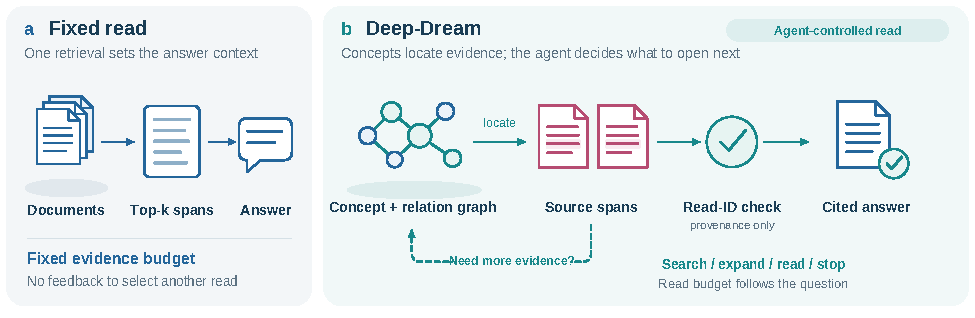
\includegraphics[width=0.98\columnwidth]{figures/fig0_motivation.pdf}
  \caption{存储与读取暴露的是不同的证据主张。可修订地址引导检索；原文段落让智能体审计措辞、身份语境和更新状态。}
  \label{fig:motivation}
\end{figure}

我们用配对构建实验、MemoryAgentBench读取路径、LongMemEval与LoCoMo历史测试，以及MEME删除检查评估两个轴。比较结果严格按协议解释：完整路径不是组件消融，同名计数只是代理指标，来源证明也不等于蕴含证明。本文贡献包括：
\begin{itemize}
    \item \textbf{校准式证据存储。} 带来源链接的观测保持可检查，推断出的身份链接可以修订。
    \item \textbf{可审计的渐进读取。} 智能体能够收集更多段落，并展示某个地址背后的证据。
    \item \textbf{双轴评估。} 在明确协议边界的前提下报告质量、覆盖、成本、对齐不确定性、图检索零结果和删除失败。
\end{itemize}

\section{相关工作}
\label{sec:related-work}

\paragraph{长期记忆基准。}
LoCoMo 和 LongMemEval 评估长对话、时序更新和多会话检索 \citep{maharana2024locomo,wu2025longmemeval}。MEME 增加删除、级联影响和缺失事实问题 \citep{jung2026meme}。MemoryAgentBench（MAB）在一个评分框架中同时测试准确检索、时序与测试时学习、长程理解和选择性遗忘 \citep{hu2025memoryagentbench}。这些基准分别覆盖存储和读取的不同部分，因此本文将它们作为互补测试，而不把长期记忆压缩成一个分数。

\paragraph{智能体记忆系统。}
MemGPT 将上下文管理描述为工作窗口与外部存储之间的分页 \citep{packer2023memgpt}。Model-Native Computing Architecture 进一步把上下文容量、缓存复用和智能体调度放在系统级资源管理框架下讨论 \citep{lin2026icam}。Mem0、Zep/Graphiti、HippoRAG-2、A-MEM、MIRIX 和 Cognee 使用摘要、笔记、图或它们的组合来保存跨会话信息 \citep{chhikara2025mem0,rasmussen2025zep,gutierrez2025hipporag2,xu2025amem,wang2025mirix,markovic2025cognee}。这些系统在“什么被保存为记忆”上各有不同：Deep-Dream 保留源文档，并把概念和关系作为指向源文档的链接，因此图中的派生节点是检索入口，而不是替代事实。

\paragraph{时序与版本化知识。}
时序知识图谱表示不断变化的实体和关系；概率记录链接则区分错误合并与漏匹配 \citep{fellegi1969theory}。Deep-Dream 将这些思想用于智能体记忆：处理时间排列观测和版本，延迟对齐使候选身份在证据充分之前保持可修订，源文本则始终保持不变。事件日期仍然属于观测内容，可以参与检索，但不会另建一套状态时钟。

\paragraph{压缩、检索与证据。}
信息瓶颈和率失真理论研究紧凑表示与目标信息之间的取舍 \citep{tishby2000information,shannon1959coding}。联想记忆研究如何从部分线索中检索内容 \citep{ramsauer2021hopfield}，检索增强生成则从外部来源选择生成证据 \citep{lewis2020rag}。长上下文模型在相关片段埋藏于大窗口中时可能丢失信息 \citep{liu2024lost}；归因研究检查回答是否引用了来源 \citep{gao2023alce}。Deep-Dream 将这些思想放入持久化记忆：概念和关系缩小搜索范围，源文本保留原始措辞，智能体决定读取多少内容；第~\cref{sec:information-view} 节给出这一分工的形式化分析。

\paragraph{智能体检索。}
A-RAG 将关键词、语义和片段读取工具交给推理模型，用于多跳检索 \citep{du2026arag}。Deep-Dream 同样允许模型选择下一步读取动作，但面向的是不断变化的个人历史。它进一步需要处理身份修订、版本链接、跨文档 Episode 和基于原文的验证。

\section{Deep-Dream}
\label{sec:deep-dream}

\subsection{记忆表示}

设 $\mathcal D_t$ 是截至处理时刻 $t$ 已处理的文档集合。对 $D\in\mathcal D_t$，设 $\mathcal E(D)$ 是从该文档不可修改的原文片段中切分出的 Episode。对 $e_i\in\mathcal E(D_i)$，定义一条存储观测为
\[
o_i=(D_i,e_i,\tau_i,x_i,\ell_i),
\]
其中 $\tau_i$ 是处理时间，$x_i$ 是抽取出的内容和属性，$\ell_i$ 是它在 $D_i$ 中的精确原文位置。写入 $t$ 条观测后的观测库为 $O_t=\{o_1,\ldots,o_t\}$。持久化状态为
\[
M_t=(F_t,O_t,G_t),
\]
其中 $F_t$ 保存概念实体族和候选身份，$G_t$ 保存关系、邻域与版本指针。每条观测都携带文档和 Episode 标识 $(D_i,e_i)$，用它们可以重新定位原文。

一次写入状态转移表示为
\begin{equation}
\begin{aligned}
F_{t+1}&=\mathsf{Align}(F_t,x_{t+1}),\\
O_{t+1}&=O_t\cup\{o_{t+1}\},\\
G_{t+1}&=\mathsf{Link}(G_t,F_{t+1},o_{t+1}),\\
M_{t+1}&=(F_{t+1},O_{t+1},G_{t+1}).
\end{aligned}
\label{eq:state-transition}
\end{equation}
这里 $\mathsf{Align}$ 要么把 $x_{t+1}$ 分配到已有实体族，要么先保留一个新的候选实体族；$\mathsf{Link}$ 在实体族、观测和版本之间增加或重定向指针。两种操作都不会修改 $\ell_{t+1}$ 所指向的原文。由于版本指针保留了早期状态，沿版本链定义的投影 $\pi_t$ 可以从 $M_{t+1}$ 恢复 $M_t$；所以状态更新是增加链接，而不是删除早期观测。

这种表示把“找到”与“读取”分开。解析实体族或关系属于索引查询，打开对应的源文本则是单独的读取操作。关系边帮助智能体找到相连的观测，但支撑这条边的陈述仍保存在原文中。处理时间 $\tau_i$ 是图谱唯一的状态轴。原文中的事件日期可以放在 $x_i$ 中并参与回答，但不会产生第二套版本时钟。

\subsection{写入记忆}

写入遵循\cref{eq:state-transition}中的状态转移：按照原文位置切分文档中的 Episode；从每个 Episode 中抽取实体和关系；将候选身份与已有概念实体族比较；最后把确认的链接和支撑它们的观测一起写入。每条链接都能沿路径回到具体文档片段。

首次提及无法确定实体身份时，Deep-Dream 会先保留多个候选实体族。后续观测和关系邻域提供足够证据后，再合并兼容的实体族或重定向指针。这个操作只修改 $F_t$ 和 $G_t$，不修改 $O_t$ 中的观测。因此，暂时拆分可以在之后修正；相反，过早合并可能把两段历史混在同一个检索入口下。

\subsection{即时对齐与延迟实体对齐}

实验比较两种写入时机，它们使用相同的状态表示。 \textbf{即时对齐（Base）} 在每个窗口到达时执行 $\mathsf{Align}$；\textbf{延迟对齐（Align+）} 先追加 $o_i$ 和候选链接，等周围窗口处理完后再解析兼容的实体族。两者的区别在于身份决策何时发生，而不是图谱结构或原文记录不同。

延迟对齐在做合并之前使用更多上下文。它可以把兼容候选放在一起处理，减少重复工作，同时保留支撑每次决策的源文本。第~\cref{sec:temporal-benchmark} 节的配对结果量化了这种取舍。

\subsection{读取记忆}
\label{sec:answer-paths}

设 $\mathcal S_t$ 是 $M_t$ 中全部不可修改的源文本片段。对问题 $q$，智能体从 $C_0(q)=\varnothing$ 开始，选择动作
\[
a_{k+1}=\rho\bigl(q,M_t,C_k(q),u_k\bigr)
\in\bigl(\mathcal S_t\setminus C_k(q)\bigr)\cup\{\mathsf{stop}\},
\]
其中 $u_k$ 是智能体当前的不确定性。如果 $a_{k+1}$ 是一个源文本片段，就打开它并令
\[
C_{k+1}(q)=C_k(q)\cup\{a_{k+1}\};
\]
如果 $a_{k+1}=\mathsf{stop}$，读取过程结束。用归纳法——每一步只把 $\mathcal S_t$ 中的一个片段加入 $C_k$——可得 $C_k(q)\subseteq\mathcal S_t$ 且 $C_k(q)\subseteq C_{k+1}(q)$。这个公式只记录打开源文本的动作；词法、语义、概念和关系查询会更新 $u_k$，但不会把片段加入 $C_k$。这就是渐进读取的形式化定义；何时停止由策略决定。

提问时，智能体从当前最有用且成本较低的线索——词法、语义、概念或关系——开始，打开对应 Episode 或源文本，在证据不完整时继续扩展：只问一个事实时，可能一段原文就够了；涉及更新或多个文档时，则可能需要沿关系和版本链接继续读取。

我们比较三种读取方式：
\begin{enumerate}
    \item \textbf{固定检索。} 只运行一次词法/语义/图检索，把一份排序后的记忆记录和检索片段交给答题模型；列表不能再修改，也不会与源文件核对。
    \item \textbf{工具辅助读取。} 把只读的搜索、概念、关系和片段工具交给答题智能体；它可以多次调用，并用一次结果组织下一次查询，但答题模型拿到的是工具返回的记录。
    \item \textbf{原文读取。} 用索引选择文档组，再打开原始文件、读取精确片段，并且只提交通过原文门禁的片段。
\end{enumerate}

源文本检查器确认引用的标识符确实由工具返回，并且仍然指向原文。它保证引用来源可追溯，但仍需要智能体判断该片段是否真正支持答案。

\subsection{为什么这种表示能够保留有用细节}
\label{sec:information-view}

设 $Z$ 是观测对应的潜在实体身份。由于 $\pi_t(M_{t+1})=M_t$，较新的状态包含早期状态，以及新观测和修订后的链接。因此
\begin{equation}
\begin{aligned}
H(Z\mid M_t)-H(Z\mid M_{t+1})
&=I(Z;M_{t+1}\mid M_t)\\
&\ge 0.
\end{aligned}
\label{eq:state-uncertainty}
\end{equation}
第一个等式成立是因为 $M_t$ 可以由 $M_{t+1}$ 恢复——这是由保留的版本链接提供的表示不变量，并不是任意图边都能推出的。如果新观测不含有区分 $Z$ 的信息，差值就是零；如果它能区分候选实体族，条件熵就会下降。这是保留状态的结构性保证，不是已经测量得到的熵增益。

对于问题 $q$，设 $A$ 是用于定位候选的紧凑记录，$E_C$ 是从候选集合 $C$ 中打开的源文本，$Y$ 是与答案有关的事实。链式法则给出
\begin{equation}
I(Y;A,E_C\mid Q=q)=I(Y;A\mid Q=q)+I(Y;E_C\mid A,Q=q).
\label{eq:two-rate-code}
\end{equation}
这就是链式法则。第一项表示定位候选时使用的信息，第二项表示读取源文本后获得的额外信息。Deep-Dream 压缩的是检索描述，而不是事实的唯一副本。

设 $R_q$ 表示相关源文本位于已打开集合 $C_K(q)$ 中，设 $V_q$ 表示最终答案正确，即 $V_q=\{\widehat Y=Y\}$。由全概率公式，
\begin{equation}
\begin{aligned}
\Pr[\widehat Y=Y\mid q]
&=\Pr[R_q\mid q]\Pr[V_q\mid R_q,q]\\
&\quad+\Pr[\neg R_q\mid q]\Pr[V_q\mid\neg R_q,q]\\
&\ge \Pr[R_q\mid q]\Pr[V_q\mid R_q,q].
\end{aligned}
\label{eq:answer-decomposition}
\end{equation}
概念和关系链接主要影响第一项，原文读取和引用检查影响第二项。这个不等式不是性能估计，只是把正确回答分解为“找到相关证据”和“读取后正确作答”两个环节。

\section{实验}
\label{sec:experiments}

我们分别评估两项操作：在历史不断增长且身份可修订的情况下保存记录，以及针对问题读取所需的证据。

\subsection{评估设置}
\label{sec:setup}

我们使用四个公开基准。主要的MemoryAgentBench（MAB）评估包含10个任务组、59份文档和767道配对题；Align+扩展到14个任务组、1{,}074道题（完整集合为29个任务组、3{,}671道题）。所有MAB分数均由官方评分器\footnote{本轮实验固定使用提交\texttt{455306d}的评分器。}计算，回答模型为Kimi-K3。LongMemEval先写入完整对话集合，再用配对的$n{=}25/25/27$样本运行三种回答方法。MAB以百分比报告（100表示全部正确，0表示全部错误）；AR为\emph{Accurate Retrieval}，TTL为\emph{Test-Time Learning}，LRU为\emph{Long-Range Understanding}，SF为\emph{Selective Forgetting}；MCC为\emph{Multi-Class Classification}，Recom为按Recall@5评分的电影推荐，FC-SH/FC-MH分别为单跳和多跳FactConsolidation。Recall、$J$、exact-match和Overall均为越高越好，calls、tokens和bytes为成本指标。采样与评审细节见附录~\ref{app:sampling}，附录表~\ref{tab:experiment-map}说明各基准对应存储问题还是读取问题。

\begin{figure*}[t]
  \centering
  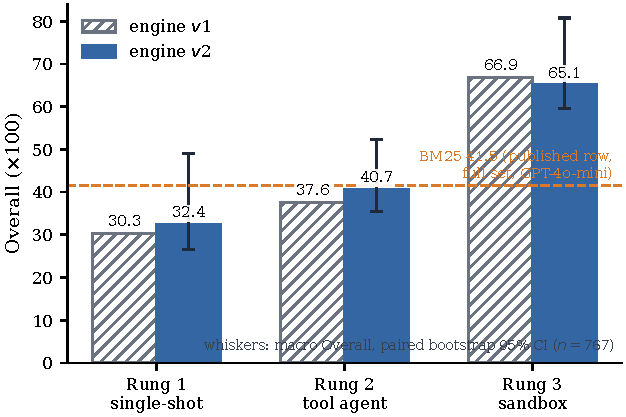
\includegraphics[width=\textwidth]{figures/fig2_ladder.pdf}
  \caption{MemoryAgentBench results by method and task (official scorer, Kimi-K3 answerer). (a) Overall scores: Base on the frozen paired sample ($n{=}767$), Align+ on the extended sample ($n{=}1074$), with marginal 95\% bootstrap intervals; (b) Align+ domain scores at the extended sample; (c) selected task scores; (d) all 209 residual zero-score items of the extended sample. The two sample definitions are labeled separately.}
  \label{fig:ladder}
\end{figure*}

\subsection{如何存储：更新与实体对齐}
\label{sec:temporal-benchmark}
\label{sec:engine-versions}
\label{sec:engine-paired}
\label{sec:deletion-boundary}

LongMemEval检验完整对话历史写入后，早期陈述和后续修正是否都能被找到。在配对运行中，直接检索由0.68升至0.72，记忆工具阅读由0.68升至0.72，原文支撑阅读由0.889升至0.926（$n{=}25/25/27$；这些轨迹样本较小，只能作方向性观察）。这些配对运行表明，新旧观测可以由同一读取路径共同访问。独立的500题LongMemEval-S运行达到84.60\%，回答者和评审均为Qwen3.7-plus；该协议与表中其他回答者/评审组合不同。

对齐实验检验身份何时被最终确定。即时对齐逐窗口决策，延迟对齐则等待周围证据。在配对写入记录中，每份MAB文档的调用由609降至329，每份LongMemEval文档由63.8降至22.0。同名重复族在MAB上由340降至124，在LongMemEval上由482降至99。配对样本中MCC和FC-MH各提高3个百分点，95\%区间为$-7$至$+13$（包含零）。这些数据对应一个组合式写入路径，其中同时使用延迟对齐、批处理和并发处理；实际效果是降低构建成本，并为修订身份链接提供更多机会。三臂分解见附录表~\ref{tab:alignment-ab}，附录图~\ref{fig:alignment-outcomes}分别展示成本、重复族和质量变化。

MEME把历史保留与删除区分开来：100个episode共进行694次后任务检查，删除准确率为0\%，级联为46.34\%，缺失为59.23\%。这个零值是当前写入/读取路径的属性：MEME删除事件要求系统停止返回某条旧事实，同时保留周围历史；测试路径却把删除陈述记录为另一条观测，没有墓碑标记，也没有从实体或关系传播到受影响片段的查询时抑制规则，因此证据虽被保留，仍会被检索。支持删除需要记录删除目标，把不可用状态传播到派生指针，并区分当前查询与历史查询。这个结果精确定位了缺失操作，不能说明仅靠保留来源就实现了遗忘。对应的更新、邻居跳转和删除分解见附录图~\ref{fig:diagnostics}。

\subsection{如何读取：渐进式证据检索}
\label{sec:ladder}
\label{sec:relational-benchmark}

图~\ref{fig:ladder}给出分面板结果。面板(a)在Align+上约由33升至40再升至71；面板(b)显示原文路径达到88.8 AR、52.9 TTL、62.3 LRU和80.0 SF，而其他路径的TTL仍为2.6。面板(c)在MCC（46.0）和FC-MH（70.0）上呈现相同优势；面板(d)显示209道零分题中有122道属于TTL。因而，增益与原文访问以及围绕更新和事实整合的持续取证有关。

三条路径（\cref{sec:answer-paths}）在答案者获得的内容和追加请求的权限上不同。\textbf{固定检索}一次性生成记忆记录和分块的排序列表，不能修改、重新打开或核对。\textbf{记忆工具阅读}可以多次发起只读调用，第二次调用可利用第一次返回的实体或关系，但答案者的上下文局限于工具返回的记录，没有来源文件门。\textbf{原文支撑阅读}用同一索引选择文档组，再打开原始文件，只把通过来源门的片段交给答案者。因此，第二条路径是在存储记录上的自适应导航，第三条路径则在此基础上增加原文阅读。

逐行结果呈现相同模式：原文阅读在MCC、FC-MH、MH-QA和LongMemEval-S上最强，而工具阅读主要帮助DetectiveQA等任务。这些任务中，第一段看似相关的分块并不够用，智能体必须合并多次提及、追踪更新或核对限定词。固定路径无法请求缺失提及；工具路径可以请求另一条有界记录；原文路径能够检查所选文件并核对措辞。614题热图和路径协议对比见附录图~\ref{fig:alignment}与附录表~\ref{tab:answer-path-differences}。

全文参考在文档组适合预算的614道题上达到78.7。原文支撑阅读在相同题目上为70.8，在扩展的1{,}074题上为71.0，并且仍可处理超出预算的460道题。全文上下文在能够容纳时表现很强，而地址化读取可以在语料超过单一窗口后继续工作。

LoCoMo在Mem0兼容的二元$J$指标下测试跨Episode证据（即由语言模型评审判定为正确的答案比例）。Deep-Dream总体达到95.19\%（单跳97.38，多跳93.62，开放域80.21，时间95.33），独立的Qwen3.7-plus交叉评审在同一答案上给出94.22\%。由于1,540行中有1,529行早于运行时代码指纹记录，我们将其作为单次诊断；已发表的Mem0和Zep行保留各自的回答者、评审者和测试流程。多跳与时间结果与设计相符：关系路径连接Episode，来源观测保留支撑陈述。

\begin{table*}[t]
\centering
\footnotesize
\setlength{\tabcolsep}{4.5pt}
\renewcommand{\arraystretch}{1.12}
\begin{tabular*}{\textwidth}{@{\extracolsep{\fill}}lrrrrrrr@{}}
\toprule
 & \multicolumn{2}{c}{Direct retrieval}
 & \multicolumn{2}{c}{Tool-assisted reading}
 & \multicolumn{2}{c}{Source reading}
 & \multicolumn{1}{c}{\shortstack{Source$-$Direct\\(Align+)}} \\
\cmidrule(lr){2-3}\cmidrule(lr){4-5}\cmidrule(lr){6-7}\cmidrule(lr){8-8}
Task / domain
 & Base & Align+ & Base & Align+ & Base & Align+
 & \shortstack{Source$-$Direct\\(Align+)} \\
\midrule
\rowcolor{blue!10}
\multicolumn{8}{@{}l}{\textbf{AR: Accurate Retrieval}} \\
SH-QA
 & 54.0 & 48.0 & 84.0 & 72.0 & \textbf{94.0} & \underline{92.0} & 44.0 \\
MH-QA$^{\ddagger}$
 & -- & 22.0 & -- & \underline{42.0} & -- & \textbf{77.0} & 55.0 \\
LongMemEval-S$^{*}$
 & 26.7 & 41.7 & 43.3 & 51.7 & \textbf{90.0} & \underline{88.3} & 46.6 \\
EventQA
 & \underline{90.3} & 89.7 & \underline{90.7} & 88.3 & \textbf{98.0} & \textbf{98.0} & 8.3 \\
\midrule
\rowcolor{green!10}
\multicolumn{8}{@{}l}{\textbf{TTL: Temporal and Test-time Learning}} \\
MCC, icl\_clinic150
 & 4.0 & 2.0 & 3.0 & 2.0 & \underline{43.0} & \textbf{46.0} & 44.0 \\
Recom$^{\ddagger}$
 & -- & \underline{3.2} & -- & \underline{3.2} & -- & \textbf{59.8} & 56.6 \\
\midrule
\rowcolor{orange!12}
\multicolumn{8}{@{}l}{\textbf{LRU: Long-range Understanding}} \\
$\infty$Bench-Sum$^{\dagger}$
 & 0.0 & 0.0 & \underline{28.4} & \textbf{29.8} & 21.2 & 0.0 & 0.0 \\
DetectiveQA
 & 50.0 & \underline{66.7} & 50.0 & \textbf{83.3} & \textbf{83.3} & \textbf{83.3} & 16.6 \\
\midrule
\rowcolor{purple!10}
\multicolumn{8}{@{}l}{\textbf{SF: Selective Forgetting}} \\
FC-SH
 & \underline{68.0} & 66.0 & 67.0 & 63.0 & \textbf{90.0} & \textbf{90.0} & 24.0 \\
FC-MH
 & 2.0 & 3.0 & 4.0 & 4.0 & \underline{67.0} & \textbf{70.0} & 67.0 \\
\midrule
\rowcolor{gray!12}
\textbf{Overall ($n=767$)}
 & 30.2 & 32.4 & 37.6 & 40.7 & \textbf{66.9} & \underline{65.1} & 32.7 \\
Overall ($n{=}1074$, extended)
 & -- & 33.3 & -- & 40.0 & -- & \textbf{71.0} & 37.7 \\
\bottomrule
\end{tabular*}
\caption{MemoryAgentBench scores (percent). The last column is Source$-$Direct within Align+; it is reported when both Align+ paths are available. Bold and underlining mark the best and second-best entry within each row.}
\label{tab:main-results}
\end{table*}



\begin{figure*}[t]
  \centering
  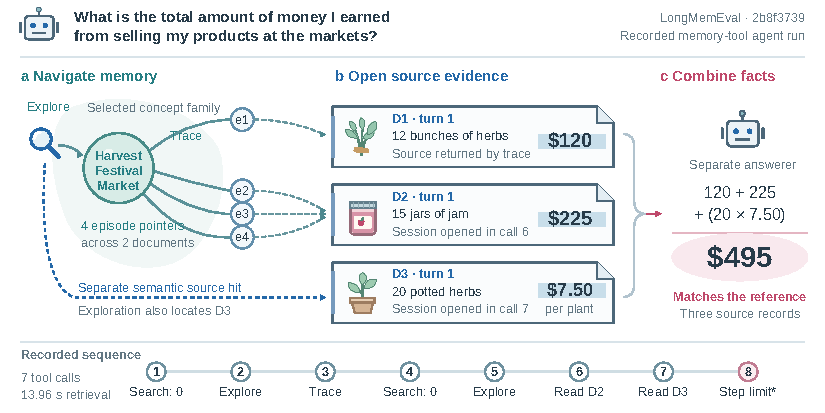
\includegraphics[width=0.88\textwidth]{figures/fig4_agent_trace.pdf}
  \caption{Recorded LongMemEval trace (question \texttt{2b8f3739}): concept tracing exposes four episode pointers across two documents, and semantic retrieval locates the third sales record. Seven successful calls read $120$, $225$, and $7.50$; a malformed eighth response reaches the step limit, after which a separate answerer computes $495$. The trace shows graph navigation locating candidates and source spans supplying the arithmetic.}
  \label{fig:agent-trace}
\end{figure*}


一个实际的LongMemEval轨迹具体展示了存储结构和读取过程如何衔接。智能体先沿着概念和关系指针跨越两份文档，再打开包含\$120、\$225、数量20和单价\$7.50的原文片段，计算出$120+225+(20\times7.50)=495$。七次成功调用显示图结构负责定位候选，原文片段提供算术所需的数值；第八次格式错误并达到步数上限的记录也被保留，便于审计。这个案例用于说明读取过程，不替代总体基准结果。

\subsection{与现有记忆系统的比较}
\label{sec:cross-system}

表~\ref{tab:main-cross-system}将Deep-Dream与MAB、LoCoMo和LongMemEval-S的已发表结果并列，模型列明确每种配对。在MAB行中固定使用Kimi-K3：固定检索33.3，迭代记忆工具40.0，原文阅读71.0；78.7的全文行是在文档适合窗口的614道题上的同模型参考上限。已发表行保留其原有回答者和评审者，因此只有同模型MAB配对构成受控比较。分类复现见附录表~\ref{tab:mem0-baselines}--\ref{tab:zep-longmemeval}和~\ref{tab:mem0-f1-bleu}。绿色行标记近期强模型报告：$\dagger$使用GPT-5-mini/GPT-5，$\ddagger$使用GPT-4.1-mini或GPT-5-mini并由GPT-4o-mini评审，$\ast$使用Gemini-3 Pro以及GPT-OSS-120B记忆和评审\citep{ji2026infini,wang2026memmachine,latimer2025hindsight}。LongMemEval-S上，Deep-Dream的84.6（Qwen3.7-plus回答者和评审者）低于MemMachine（93.0）、Hindsight（91.4）和Supermemory（85.2）；差距主要集中在会话偏好、时间推理和多会话问题。Deep-Dream在助手事实、用户事实和知识更新上较强；这些是下一步读取和更新的目标，同时保留MAB上的原文读取优势以及LoCoMo多跳和时间维度的表现。

对于Infini Memory-A，MAB行采用其论文报告的四类平均值：AR为81.2，TTL为51.0，LRU为68.6，SF为58.0，总体为64.7；不以更细的子任务分数替换这些类别值。

\begin{table*}[t]
\centering
\scriptsize
\setlength{\tabcolsep}{2.4pt}
\renewcommand{\arraystretch}{0.82}
{\footnotesize\textbf{(a) MemoryAgentBench (official scorer)}}\\[1.5pt]
\begin{tabular*}{\textwidth}{@{\extracolsep{\fill}}>{\raggedright\arraybackslash}p{0.25\textwidth}>{\raggedright\arraybackslash}p{0.15\textwidth}rrrrr@{}}
\toprule
Memory system & Answerer & AR & TTL & LRU & SF & Overall \\
\midrule
Full context & GPT-4o & 58.1 & 50.0 & 54.9 & 32.5 & 48.8 \\
Full context & GPT-4o-mini & 49.2 & 48.6 & 46.2 & 25.0 & 42.2 \\
Full context & GPT-4.1-mini & 71.8 & 46.2 & 49.1 & 20.5 & 46.9 \\
Full context & Gemini-2.0-Flash & 65.1 & 46.4 & 41.6 & 16.5 & 42.4 \\
Full context & Claude-3.7-Sonnet & 59.7 & 53.9 & 62.2 & 22.5 & 49.6 \\
\rowcolor{blue!9}
Full context ($n{=}614$) & Kimi-K3 & \textbf{96.8} & \textbf{75.0} & 65.2 & 78.0 & \textbf{78.7} \\
\midrule
BM25 RAG & GPT-4o-mini & 60.5 & 44.5 & 35.6 & 25.5 & 41.5 \\
HippoRAG-2 & GPT-4o-mini & 65.1 & 35.8 & 36.2 & 29.5 & 41.6 \\
MIRIX & GPT-4.1-mini & 63.0 & 35.7 & 40.5 & 11.5 & 37.7 \\
MemGPT & GPT-4o-mini & 34.3 & 40.8 & 22.4 & 15.5 & 28.3 \\
Zep & GPT-4o-mini & 37.5 & 37.5 & 16.2 & 5.0 & 24.0 \\
Mem0 & GPT-4o-mini & 32.6 & 21.2 & 20.7 & 10.0 & 21.1 \\
\rowcolor{green!9}
Infini Memory-A & GPT-5-mini$^\dagger$ & 81.2 & 51.0 & \textbf{68.6} & 58.0 & 64.7 \\
\midrule
\rowcolor{blue!9}
Deep-Dream / Direct retrieval & Kimi-K3 & 50.3 & 2.6 & 45.9 & 34.5 & 33.3 \\
\rowcolor{blue!9}
Deep-Dream / Memory-tool agent & Kimi-K3 & 63.5 & 2.6 & 60.4 & 33.5 & 40.0 \\
\rowcolor{blue!9}
\textbf{Deep-Dream / Source reading} & \textbf{Kimi-K3} & 88.8 & 52.9 & 62.3 & \textbf{80.0} & 71.0 \\
\bottomrule
\end{tabular*}

\vspace{3pt}
{\footnotesize\textbf{(b) LoCoMo $J$ score (\%; Mem0 scoring)}}\\[1.5pt]
\begin{tabular*}{\textwidth}{@{\extracolsep{\fill}}>{\raggedright\arraybackslash}p{0.25\textwidth}>{\raggedright\arraybackslash}p{0.15\textwidth}rrrrr@{}}
\toprule
Memory system & Answerer / judge & Single-hop & Multi-hop & Open-domain & Temporal & Weighted \\
\midrule
Mem0 & GPT-4o-mini & 67.13 & 51.15 & 72.93 & 55.51 & $\approx$62.14 \\
Mem0$^g$ & GPT-4o-mini & 65.71 & 47.19 & 75.71 & 58.13 & $\approx$61.36 \\
Zep & GPT-4o-mini & 61.70 & 41.35 & 76.60 & 49.31 & $\approx$56.32 \\
LangMem & GPT-4o-mini & 62.23 & 47.92 & 71.12 & 23.43 & $\approx$52.08 \\
OpenAI & GPT-4o-mini & 63.79 & 42.92 & 62.29 & 21.71 & $\approx$51.10 \\
A-Mem$^*$ & GPT-4o-mini & 39.79 & 18.85 & 54.05 & 49.91 & $\approx$38.95 \\
\midrule
\rowcolor{green!9}
MemMachine & GPT-4.1-mini / GPT-4o-mini$^\ddagger$ & 95.12 & 88.30 & 71.88 & 91.59 & 91.69 \\
\rowcolor{green!9}
Hindsight & Gemini-3 Pro / GPT-OSS-120B$^\ast$ & 86.17 & 70.83 & \textbf{95.12} & 83.80 & 89.61 \\
\midrule
\rowcolor{blue!9}
Deep-Dream (diagnostic) & Kimi-K3 & 97.38 & 93.62 & 80.21 & 95.33 & 95.19 \\
\rowcolor{blue!9}
Deep-Dream & Qwen3.7-plus / Qwen3.7-plus & 96.91 & 92.91 & 77.08 & 93.46 & 94.22 \\
\bottomrule
\end{tabular*}

\vspace{3pt}
{\footnotesize\textbf{(c) LongMemEval-S (\%)}}\\[1.5pt]
{\tiny\setlength{\tabcolsep}{0pt}\begin{tabular*}{\textwidth}{@{\extracolsep{\fill}}>{\raggedright\arraybackslash}p{0.25\textwidth}>{\raggedright\arraybackslash}p{0.15\textwidth}rrrrrrr@{}}
\toprule
Memory system & Answerer / judge & Overall & Sess. pref. & Sess. asst. & Temporal & Multi-sess. & Knowl. upd. & Sess. user \\
\midrule
Full context & GPT-4o-mini & 55.4 & 30.0 & 81.8 & 36.5 & 40.6 & 76.9 & 81.4 \\
Full context & GPT-4o & 60.2 & 20.0 & 94.6 & 45.1 & 44.3 & 78.2 & 81.4 \\
\midrule
Zep & GPT-4o-mini & 63.8 & 53.3 & 75.0 & 54.1 & 47.4 & 74.4 & 92.9 \\
Zep & GPT-4o & 71.2 & 56.7 & 80.4 & 62.4 & 57.9 & 83.3 & 92.9 \\
\rowcolor{green!9}
MemMachine & GPT-5-mini$^\ddagger$ & \textbf{93.0} & \textbf{93.3} & 98.2 & \textbf{91.7} & \textbf{87.2} & \textbf{94.9} & \textbf{100.0} \\
\rowcolor{green!9}
Hindsight & Gemini-3 Pro$^\ast$ & 91.4 & 80.0 & 96.4 & 91.0 & \textbf{87.2} & \textbf{94.9} & 97.1 \\
\rowcolor{green!9}
Supermemory & Gemini-3 Pro$^\ast$ & 85.2 & 70.0 & 98.2 & 82.0 & 76.7 & 89.7 & 98.6 \\
\midrule
\rowcolor{blue!9}
\textbf{Deep-Dream} & \textbf{Qwen3.7-plus / Qwen3.7-plus} & 84.6 & 53.3 & \textbf{100.0} & 84.2 & 74.4 & 91.0 & 98.6 \\
\bottomrule
\end{tabular*}}
\caption{Results for Deep-Dream and published memory systems on MemoryAgentBench, LoCoMo, and LongMemEval-S. Each row retains its answerer, judge, subset, and evaluation setting. The Deep-Dream LoCoMo row is a single-run diagnostic; its legacy-fingerprint details are in the appendix. Bold marks each column's maximum among the reported comparable rows; the single-run diagnostic row is intentionally unbolded; the Infini Memory-A row uses the category averages reported in its paper.}
\label{tab:main-cross-system}
\end{table*}



现有系统使用不同的记忆对象：抽取的原子记忆（Mem0）、带有效期窗口的情景图（Zep/Graphiti）、段落图（HippoRAG-2）、链接笔记（A-MEM）或类型化模块（MIRIX）。Deep-Dream保持来源片段的权威性，并以概念和关系作为可修订地址，使智能体能够在原始文件中核验多次提及的答案。

\subsection{检索与证据诊断}
\label{sec:external-comparisons}
\label{sec:provenance-ablation}

我们在相同的210道题上重放四种索引：对原始Episode使用关键词（BM25），再依次加入语义链接、图邻居和关系链接。Recall-any@10询问前十项中是否出现至少一条相关项；Recall-all@10询问是否出现全部相关项。Recall-any@10分别为72.38、72.38、71.43和72.38\%；每个配对差异都落在基于同一重放计算的$\pm$2.4个百分点95\% bootstrap等价界内，其他指标也没有稳定变化。因此，重放没有证据表明图链接单独提升离线召回；它只说明离线检索，而在线阶段实际使用了图的导航作用——在原文阅读前选择文档组、版本和关系链接——并未对该作用做消融。

附录图~\ref{fig:cost}报告相应的调用和token成本。原文支撑阅读由于需要核验并扩展证据，调用更多；但在需要多次提及或更新的问题上也产生最强答案。

\section{分析与局限}
\label{sec:analysis}

核心主张是校准存储与读取之间的关系。来源片段是被保存的观测；身份族、关系或版本是推断得到的访问结构；检索到的段落则是智能体主动选择检查的内容。把这些类别分开可以支持修订，但不能保证身份正确，也不能保证读到的段落蕴含答案。来源门只验证来源，不验证身份或蕴含关系。

这种存储选择在提出具体问题之前就决定了信息能否保留。只保存摘要会提前压缩历史，后来的问题可能需要摘要中被省略的限定条件、旧状态或原始措辞。Deep-Dream保留来源观测，把图结构只用于定位，因此当前值仍然可以回到产生它的历史观测，而不是覆盖这些观测。

延迟对齐让这种表示可以修订。过早合并可能把两个同名的人放在同一个地址下，污染双方的历史；暂时拆分只增加候选，之后可以通过重定向链接来修正。因此，入库实验说明的是成本和可修订性变化，并不能证明当前身份标签已经完全正确。版本链接还保留了当前值的形成过程：处理时间排列存储状态，原文中提到的日期仍属于观测内容。查询可以要求最新值，也可以要求较早的值，而不必改写历史记录。

Align+使写入调用减少46--65\%，但其中同时包含延迟对齐、批处理和并行处理。同名族在MemoryAgentBench上由340降至124，在LongMemEval上由482降至99。同名重复代理不是身份标签，配对质量区间为$-7$至$+13$个百分点。MCC和FC-MH各提高3个百分点，95\%区间为$-7$至$+13$，因此这些结果说明的是构建成本与可修订性的权衡，而不是身份准确率提升。熵论证还以固定目标和保留前驱状态为条件。

MAB路径比较中，固定检索、记忆工具和原文阅读在1,074道题上的Kimi-K3得分分别为33.3\%、40.0\%和71.0\%。三条完整路径在工具、原文访问、迭代方式、证据处理和预算上均有差异，因此不能据此单独分离身份层或图结构的作用。原文阅读在相同的614题上为70.8\%，全文上下文为78.7\%；另有460道题超出全文预算。离线图消融没有稳定收益。即使活动上下文较小，反复检索也可能提高成本；来源检查也不能解决停止时机或答案支持问题。

MEME在694次后任务检查中的100个删除检查上准确率为0\%，级联和缺失准确率分别为46.34\%和59.23\%。该路径没有目标级墓碑标记和传播式抑制。LongMemEval-S在Qwen3.7-plus同时担任回答者和评审时为84.6\%，协议与其他结果不同。LoCoMo的95.19\%和94.22\%是历史单次诊断，其中1,540行有1,529行早于运行时代码指纹记录。这些结果要求直接标注身份、检查蕴含关系，并开展资源匹配的读取实验。

\paragraph{尚未测量的内容。} 通过来源检查的段落仍可能与问题无关，正确链接的身份也可能需要另一份文档。当前实验没有带标签的身份决策、蕴含标注或资源匹配的停止曲线，删除结果也没有测试完整的抑制设计。后续评估应标注候选合并，在读取策略之间固定调用数和token数，并分别评价当前查询与历史查询。

\\section{结论}
\\label{sec:conclusion}

长期记忆有两个相互关联的问题：如何在实体和事实不断变化时保存不断增长的记录，以及如何在上下文窗口有限时只读取当前问题需要的证据。Deep-Dream通过保留文档片段作为事实记录，并把概念、关系、观测、版本和候选身份作为可修订的访问结构，回答了记忆如何存储的问题。读取时，智能体沿着这些结构打开相应的原文，比较早期和后续观测，并在证据足够时停止。

这种分工让每一部分承担清晰的责任。图结构缩小搜索范围，但本身不授权答案；原文片段提供具体措辞，但单独不能解决身份判断；智能体决定是否还需要查看另一份文档、关系或版本。MAB中的结果因此体现了完整读取路径的差异，而不是单独的图结构或原文消融。写入实验也表明，延迟对齐和并行处理可以降低构建成本并减少重复实体族，但目前没有测得一致的对齐质量提升。全文上下文在匹配题目上仍然更强，而MEME结果说明，保留历史记录并不等于已经规定了何时应当抑制历史。

正文中的实际轨迹进一步说明了这种分工：概念和关系负责定位候选，原文片段提供计算所需的具体数值。

本文的核心贡献，是把记忆存储和记忆读取分成两个可以分别改进、分别审计的问题：原文保留事实，概念、关系和版本提供可修订的索引，智能体自主决定读取路径和深度。后续研究可以在此基础上标注身份判断，使用相同资源评估蕴含和停止策略，并加入明确的当前状态、历史状态和删除抑制规则。


\newpage
\section*{AI 协助}
\label{sec:ai-assistance}

我们使用了基于 LLM 的协助（包括 OpenAI Codex）来起草、重构和编辑手稿；准备中文阅读版；检索相关文献与书目信息；以及协助分析与绘图代码。生成式图像工具用于创建和修改解释性框架图。

AI 协助还参与了架构的信息论解释、数学主张及其论证的表述，以及实验方法与结果的讨论。这包括渐进式实体对齐的处理、检索——证据分离，以及依赖查询的读取预算。这些论证以论文中声明的假设为条件；AI 协助不构成独立的证明验证或实证校验。

本论文准备流程中未创建任何合成评测数据集。报告的基准分数取自有记录的实验运行，而不是生成的性能估计。作者对最终文本、引用、数学主张、代码、图表和实证结论负责，包括对 AI 协助材料的核验。


\bibliography{references}
\bibliographystyle{iclr2027_conference}

\newpage
\appendix
\section{可复现性与审计细节}

\subsection{工件账本}
\label{app:ledger}

机器可读账本由发布的账本脚本与重算脚本生成。它记录论文所引每一次运行的源摘要、数据集与逐题 JSONL SHA-256 值，并在论文写作前重新生成、与脚本输出逐字节比对。当前账本覆盖 MemoryAgentBench 各轨道（两代引擎 $\times$ 三条答案路径、commit 455306d 处的官方评分器、一致的 \texttt{entity2id} 指纹）、LongMemEval 整批对话写入后的配对运行与 500 题运行、LoCoMo-1986/1540 及 K3 作答诊断、LoCoMo-Plus-401 \citep{li-etal-2026-locomo}、X7 通道诊断、源扩展诊断、修复后的预算前沿重放、MEME、BigCodeBench \citep{zhuo2024bigcodebench} 与 ALFWorld \citep{shridhar2021alfworld}。每次运行的清单记录数据集与提示词来源、模型标识符、工具观测、证据 ID、延迟、退出状态与代码/运行时哈希；未通过完整性检查的结果与负面结果均予保留而非丢弃。账本生成与重算脚本随发布的补充材料一同提供，因此该链条可端到端重建。

发布的补充材料包含重建每张表所需的机器可读清单、逐题分数、提示词与运行时哈希。论文在每个结果旁报告数据集、模型、评审、子集与完整性状态，使比较保持可审计，同时不暴露机器特定的存储位置。

\begin{figure*}[t]
  \centering
  
\includegraphics[width=\textwidth]{figures/fig1_architecture.pdf}
  \caption{Deep-Dream 的文档优先时序概念图谱。多份文档保留各自的会话片段，并通过共享的概念族与关系边连接。选中一个族会暴露其按观测时间排列的版本链，以及每次修订的精确源跨度；不确定的匹配可以先保持分离，等到后续内容与关系上下文到达时再收敛。}
  \label{fig:architecture}
\end{figure*}

\begin{figure*}[t]
  \centering
  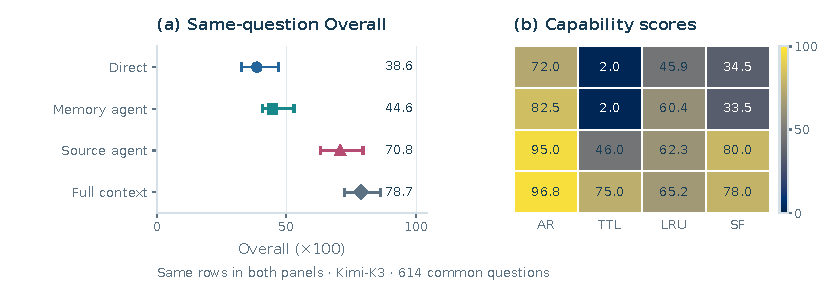
\includegraphics[width=\textwidth]{figures/figA_alignment.pdf}
  \caption{同模型完整上下文参照覆盖的 $n{=}614$ 题上的同题对齐（Kimi-K3 作答；官方宏平均评分器）。（a）带边缘 95\% bootstrap 区间的 Overall 分数；原文读取方式低于参照 $7.9$ 个百分点 [95\% CI $-11.9$, $-3.9$]。（b）域画像：参照的领先集中在 TTL，而原文读取方式在 AR、LRU、SF 上与参照持平或反超。}
  \label{fig:alignment}
\end{figure*}

\begin{figure*}[t]
  \centering
  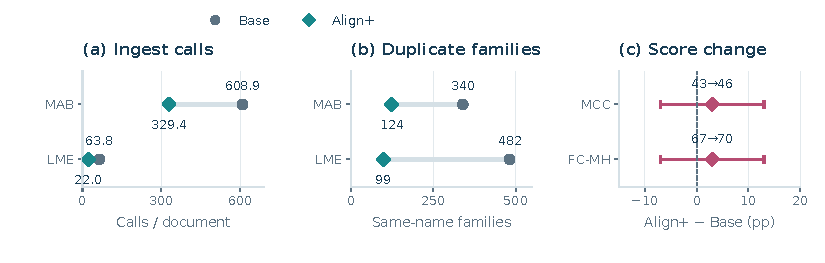
\includegraphics[width=\textwidth]{figures/figB_alignment_outcomes.pdf}
  \caption{捆绑的 Base$\to$Align+ 修订的配对构建诊断。（a）入库调用与同名重复实体族在记录在案的 MAB 与 LongMemEval 交集上下降。（b）配对的 MCC 与 FC-MH 切片各上升 3 个百分点；区间保留，因为这是捆绑比较而非组件消融。}
  \label{fig:alignment-outcomes}
\end{figure*}

\begin{table*}[t]
\centering
\small
\setlength{\tabcolsep}{3.5pt}
\begin{tabular}{@{}p{0.15\textwidth}p{0.23\textwidth}p{0.25\textwidth}p{0.30\textwidth}@{}}
\toprule
\textbf{属性} & \textbf{直接检索} & \textbf{工具辅助读取} & \textbf{原文读取} \\
\midrule
源访问 & top-$k$ 跨度 & 派生记录 & 逐字源文件 \\
工具 & 无 & 记忆工具 & 读取、grep、脚本 \\
答题模型 & 独立 & 独立 & 带验证的智能体 \\
循环 & 无 & 多次只读调用 & 多次读取并核对 \\
每题成本 & \DirectRetrievalCost & \MemoryToolCost & \SourceGroundedCost \\
\bottomrule
\end{tabular}
\caption{三种读取方式的差异。三条路径共享冻结库、问题流、Kimi-K3 与官方评分器。}
\label{tab:answer-path-differences}
\end{table*}

\begin{figure*}[t]
  \centering
  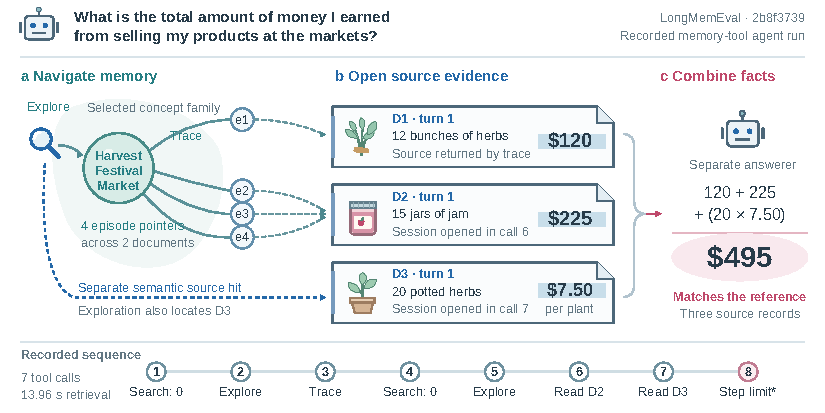
\includegraphics[width=\textwidth]{figures/fig4_agent_trace.pdf}
  \caption{一条实测 LongMemEval 轨迹（问题 \texttt{2b8f3739}）：概念追踪暴露出跨两份文档的四个会话片段指针，另一次语义命中定位到第三条销售记录。七次成功调用耗时 13.96\,s；第 8 步在一次格式错误的响应后达到上限，随后一个独立的答题模型算出 $120+225+(20\times7.5)=495$。}
  \label{fig:agent-trace}
\end{figure*}

\begin{table*}[t]
\centering
\small
\setlength{\tabcolsep}{2.5pt}
\renewcommand{\arraystretch}{1.16}
\begin{tabular*}{\textwidth}{@{\extracolsep{\fill}}p{0.04\textwidth}p{0.25\textwidth}p{0.65\textwidth}@{}}
\toprule
\textbf{RQ} & \textbf{记忆能力} & \textbf{基准与可观测预测} \\
\midrule
1 & 逐步读取原文 & MemoryAgentBench 在相同的 767 题上比较直接检索、多次调用只读记忆工具与读取原文并核对引用。当智能体可以持续阅读时，分数应当在事实整合与多次提及任务上拉开最大。 \\
2 & 时序与多会话访问 & LongMemEval 测试更新与跨会话链接。版本化观测应让较早与较晚的事实都仍然能被找到，而偏好问题仍是潜在用户状态建模的边界。 \\
3 & 关系整合 & LoCoMo 区分单跳、多跳、时序与开放域问题。当答案需要连接多个会话片段或修订较早数值时，概念族与关系路径应当最关键。 \\
4 & 可修订构建 & Base/Align+ 配对运行度量重复族、入库调用、token 与任务切片。渐进式对齐预测更低的构建成本与更好的整合，但不要求分数全面上升。 \\
5 & 删除与缺失边界 & MEME 测试删除、级联与缺失。当前的只增存储应保留溯源，但尚不能保证删除后的抑制。 \\
\bottomrule
\end{tabular*}
\caption{研究问题与测量方式。每一行检验检索——证据分离的一条不同预测；已发表结果保留各自的测试条件，便于检查分数差异。}
\label{tab:experiment-map}
\end{table*}


\subsection{版本溯源与对齐 A/B 研究}
\label{app:alignment-ab}

随附的证据包补充了一项完整的三臂对齐研究（LongMemEval-S）：三个文档组（42+49+46 份文档，每臂 137 份文档）、先写入全部文档、同一 Kimi-K3 端点。臂 A 为不带批量候选检查的基线；B1 启用批量候选检查；B2 额外启用修订后的收敛实现（并行对齐、推迟的非破坏性合并，以及最后一致性检查）。保存的 B1 与 B2 服务配置逐字节相同；二者的差异在运行时代码与 B2 开关上，因此臂分配从清单与代码快照读出，而不是从文件名推断。该研究的统计功效面向效率与整合而非质量：每个文档组在每条评测轨道上只贡献一道题。

另一项 LME Base/Align+ 引擎差异（初始/修订实现）是从 commit $73d9c5e$ 到 $8fa9651$ 的事后重建。后者还包含四项吞吐修复，因此仅凭它无法确定 Align+ 运行中各时点哪些修复处于生效状态。我们以清单内嵌的流水线配置、运行时策略哈希与技能哈希为准；重建的差异只是未提交代码的溯源材料，并不是“每项后来的修复从首次修订运行起就已生效”的主张。

\subsection{MemoryAgentBench 抽样框与污染说明}
\label{app:sampling}

抽样子集按发布账本中记录的固定任务组清单抽取：10 个任务组、59 份文档上的 767 题配对样本，并在 Align+ 引擎上原地扩展四个任务组（RULER-421K 多跳问答 100 题；完整 Redial 推荐语料 200 题；再加一个 DetectiveQA 任务组 6 题；再加一个 $\infty$Bench-Sum 任务组 1 题）至 14 个任务组上的 1{,}074 题；完整基准为 29 个任务、3{,}671 题。四种能力全部覆盖；扩展后仍有 17 个任务未被抽样。配对样本及其 \texttt{entity2id} 指纹为全部六次运行（三条路径 $\times$ 两代）共享；307 道扩展题仅存在于 Align+；两个大型扩展文档组（190 万与 570 万字符）超出完整上下文参照 1{,}042{,}576 字符的严格预算，因此参照覆盖为 1{,}074 题中的 614 题。参照使用中性提示词档案；同一次运行的 normalized-v1 档案在其自身的 607 题覆盖上得 46.0 分——这是账本中保留的提示词敏感性痕迹，不作为参照使用。文档组长度是异质的，并在跨系统单元格领先的场合均予披露：两个事实整合（FactConsolidation）文档组是 6K 变体（各 26{,}157 字符）；32K/64K/262K 的 FC 变体（13.6 万--110 万字符）与其他未抽样文档组因预算被舍弃，全部连同上下文大小列于发布账本的子集块中；EventQA 按 64K/128K/完整文档组抽样，而非只取已发表的全本均值；LRU 域有 $n{=}7$ 道配对题与 14 道扩展题（$\infty$Bench-Sum 先 1 后 2，DetectiveQA 先 6 后 12），因此 LRU 单元格是方向性的。MAB 源语料是公开的；答题模型的预训练是否见过它们无法排除、也无法事后度量，且每一行跨系统表格都声明自己的答题模型、评审与子集。

\begin{table*}[t]
\centering
\footnotesize
\setlength{\tabcolsep}{5pt}
\renewcommand{\arraystretch}{1.08}
\resizebox{\textwidth}{!}{%
\begin{tabular}{@{}p{0.16\textwidth}p{0.31\textwidth}rrrr@{}}
\toprule
臂 & 对齐修订 & 调用/文档 & 总 token/文档 & 实体重定向 & 重复组 \\
\midrule
A & 基线 & 68.4 & 145{,}378 & 0 & 8 \\
B1 & 批量候选检查 & 24.2 & 108{,}467 & 1 & 12 \\
B2 & 批量检查 + 最后一致性检查 & 29.4 & 111{,}853 & 245 & 6 \\
\bottomrule
\end{tabular}
}%
\caption{每臂 137 份 LongMemEval-S 文档上的三臂对齐研究。B1 提供大幅效率下降；B2 在最后一致性检查上比 B1 多花约 3\% 的 token，是唯一具有实质非破坏性族重定向的臂，降低了同名重复组。质量切片太小，不足以做质量主张。B1 与 B2 使用同一份保存的服务配置；B2 的差别在运行时实现与对齐开关。}
\label{tab:alignment-ab}
\end{table*}


\subsection{调整 Overall 的推导}
\label{app:adjusted-overall}

配对样本漏掉了两个对所有人都得分很低的任务——AR 的 MH-QA 与 TTL 的推荐——早期草稿用插补处理：代入已发表的非全上下文参考值（推荐 $\approx$13、MH-QA $\approx$60）后，调整 Overall 为 $\approx$59.0，而配对样本口径的原始值为 65.1，敏感性下的区间为 59--61。扩展取代了插补：两个任务现在都在 Align+ 上直接测得（读取原文 MH-QA 77.0、推荐 59.8；\cref{tab:main-results}），扩展 Overall 为 71.0，两个任务都进入了聚合。扩展样本的构成仍与完整基准不同（17 个任务未抽样），因此我们继续只陈述原始值、绝不做跨样本口径的相减；插补估计在此保留，作为发布账本的溯源材料。


\subsection{各路径提示词与配置}
\label{app:configs}

所有路径都用 Kimi-K3 作答，提示词逐字存档于 \cref{app:ledger} 所列的运行清单与代码快照中；发布的补充材料完整重印它们。Base$\to$Align+ 的引擎配置差异如下：最大输出 token 16{,}384$\to$32{,}768；可用上下文窗口 32k$\to$262{,}144；重试 2$\to$5；超时 300\,s$\to$1{,}200\,s；Align+ 启用绝对路径持久化。直接检索做一次融合检索调用与一次作答调用；工具辅助读取会多次调用只读工具；原文读取智能体物化一个文档组、读取并验证源文件，且只提交通过引用检查的跨度。

\begin{figure}[t]
  \centering
  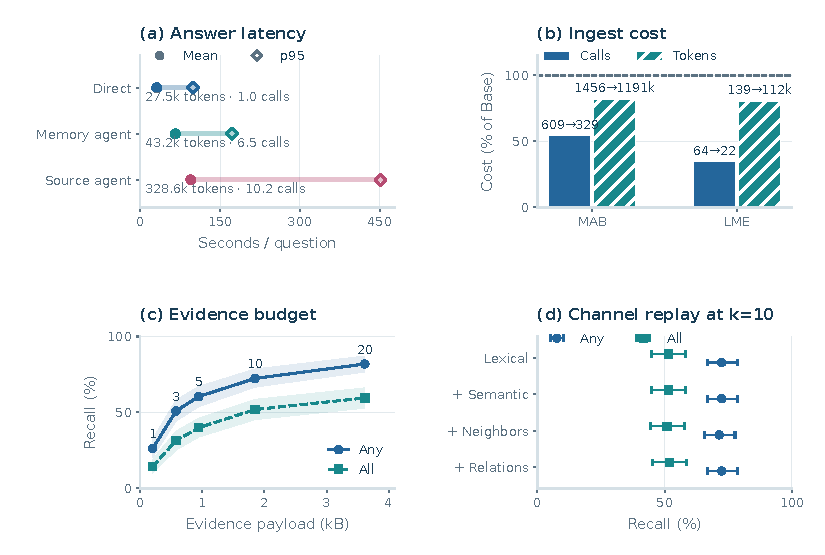
\includegraphics[width=\columnwidth]{figures/fig3_cost.pdf}
  \caption{冻结产物的运行点诊断（Align+ 引擎；面板 a 覆盖全部 1{,}074 题）。(a) 答案延迟的均值到 p95，标注 token 数与调用数；(b) 配对的 Base$\to$Align+ 入库成本；(c) 有效的固定排序检索预算前沿；(d) $k{=}10$ 处的仅源文档通道重放。}
  \label{fig:cost}
\end{figure}

\subsection{附加定量诊断}
\label{app:additional-diagnostics}

账本还包含类型级更新分数、一次受控的源扩展重放，以及 MEME 删除边界。图~\ref{fig:diagnostics} 报告这些量，并让样本量与开发集限制保持可见。

\begin{figure*}[t]
  \centering
  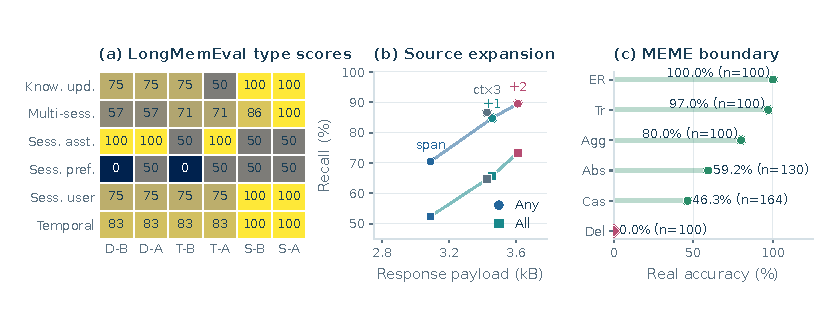
\includegraphics[width=\textwidth]{figures/figC_diagnostics.pdf}
  \caption{来自冻结账本的额外定量诊断。（a）配对 Base/Align+ 轨道的 LongMemEval 类型分数；这些方向性样本 $n{=}25/25/27$，以粗略百分比显示。（b）105 个历史错误案例上的源扩展召回对响应载荷；这是开发诊断，不是留出测试。（c）带任务特定分母的 MEME 真实任务准确率，暴露 0\% 的删除边界。}
  \label{fig:diagnostics}
\end{figure*}


\subsection{载体参照（BigCodeBench \citep{zhuo2024bigcodebench}、ALFWorld \citep{shridhar2021alfworld}）}
\label{app:carrier-anchors}

BigCodeBench：0.4859 完成率 / 0.2838 困难 pass@1（校准切分）。ALFWorld：0.9786 同分布 / 0.9851 异分布成功率。两者都是对记忆不敏感的智能体载体回归测试：它们锚定智能体载体能正确执行任务，而不与记忆基准横向比较。

\subsection{MAB 入库清单缺口}
\label{app:manifest-gaps}

Base 与 Align+ 的 MAB 入库运行共享 45 份文档的配对交集。在某一代中缺失清单的文档被排除在每文档效率比之外，因此效率比只在交集上计算（每文档调用 609$\to$329，$-46\%$）；token 比使用同一交集。题目级结果不受影响：全部 767 道配对题在两代中都对着冻结库运行，307 道扩展题只在 Align+ 引擎上运行，因此入库成本比仍定义在配对交集上。

\subsection{预算前沿}
\label{app:budget}

早期的一次 depth-10 对 depth-20 重放作为一项完整性发现被保留：其前缀不变量在全部 210 题上失败（\texttt{primary\_result\_invariant\_violations=210}），因此它不用于任何正面主张。修复后的设计对每个查询以最大深度只运行一次检索，并把固定的排序切到 $k\in\{1,3,5,10,20\}$；前缀单调性因此按构造成立（零违例），前沿从 $k{=}1$ 到 $k{=}20$ 单调上升，每个 $k$ 的百分位 bootstrap 置信区间从冻结的重放产物重新计算。

\subsection{X7 通道消融细节}

\begin{table*}[t]
\centering
\caption{X7 来源记录消融：210 题检查集上的离线检索重放。臂 1--4 构成干净的通道消融：只有 \texttt{enabled\_channels} 不同，因此任何召回差异都可归因于该通道集合。臂 5（引用核对智能体，开启检查）与臂 6（未被检索到的证据，放宽检查）复用臂 4 的五通道排序，与臂 4 检索一致；它们的区分列（问答准确率、无支撑答案率、平均证据 token）需要 LLM 智能体运行，尚待完成。引用检查流程已离线验证：开启检查时提交一个未浮现的对话轮会被拒绝；放宽检查时同一提交被接受（\texttt{plumbing\_ok}=true）。在部署的 MAB 运行中，检查按设计触发：\GateRejectStats{}。Bootstrap 置信区间：2{,}000 次重采样，95\%。}
\label{tab:provenance-ablation}
\small
\setlength{\tabcolsep}{3pt}
\begin{tabular}{llrrr}
\toprule
臂 & 通道(累加) & Recall-any@10 [95\% CI] & Recall-all@10 [95\% CI] & 平均字节@10 \\
\midrule
1 & raw-doc + episode-bm25 & 72.38 [66.67, 78.57] & 51.43 [44.76, 58.10] & 1833 \\
2 & + semantic-provenance & 72.38 [66.67, 78.57] & 51.43 [44.76, 58.10] & 1841 \\
3 & + graph-neighbor & 71.43 [65.70, 77.62] & 50.95 [44.29, 57.62] & 1845 \\
4 & + relation-evidence (full 5) & 72.38 [66.65, 78.57] & 51.90 [45.24, 58.58] & 1847 \\
\bottomrule
\end{tabular}
\end{table*}



\subsection{测试条件说明}

原始 LoCoMo token-F1 轨道含 1{,}986 题与五个类别。Mem0 兼容轨道含 1{,}540 题与四个类别。LongMemEval-S 含 500 题；整批写入后的配对运行使用 \cref{sec:setup} 所述的 $n{=}25/25/27$。MEME 的 100 个会话片段产生异质的任务数（所引运行中 ER/Agg/Tr/Del/Cas/Abs 的事后检查数为 100/100/100/100/164/130）。raw 分数与 real 分数不可互换。

\subsection{保留的完整性失败}

\cref{app:budget} 的深度重放报告 \texttt{primary\_result\_invariant\_violations=210} 且 \texttt{passed=false}。MEME 删除结果为 0\% 的 real 准确率。X7 通道消融是零结果，以等价界的形式报告而非丢弃。$\infty$Bench-Sum 的 $n{=}1$ 翻转直接使 Align+ Overall 损失 2.7 分（Base$\to$Align+ 净差距为 1.8 分），并在每处比较中披露。LongMemEval 上直接检索与工具辅助读取打平的结果虽然对记忆工具路径不利，仍予报告。这些记录保持可见，因为一篇可审计的记忆论文应当同时暴露失败与零结果的机制，而不只是成功的机制。

\subsection{外部比较协议}
\label{sec:published-baselines}

Mem0 原论文报告 LoCoMo 类别级 F1、BLEU-1 与一个二值 $J$：GPT-4o-mini 评审把每个答案标为 CORRECT 或 WRONG，得分即判定为 CORRECT 的百分比（10 次独立运行的均值$\pm$标准差）。Zep 原论文报告 DMR 与 LongMemEval，答题模型为 GPT-4o 系列。我们不在自己的协议下重跑这些系统，而是在下方逐字重印其已发表表格（表~\ref{tab:mem0-baselines}--\ref{tab:zep-longmemeval}）作为不同测试流程下的参考结果。因篇幅从正文表格中省略的 Mem0 确定性 token 重叠指标重印于表~\ref{tab:mem0-f1-bleu}。

\begin{table*}[t]
\centering
\small
\setlength{\tabcolsep}{2pt}
\renewcommand{\arraystretch}{1.12}
\begin{tabular*}{\textwidth}{@{\extracolsep{\fill}}>{\raggedright\arraybackslash}p{0.30\textwidth}>{\raggedright\arraybackslash}p{0.21\textwidth}>{\centering\arraybackslash}p{0.16\textwidth}>{\raggedright\arraybackslash}p{0.29\textwidth}@{}}
\toprule
基准 & 协议 & 分数 & 答题 / 评审 \\
\midrule
LongMemEval-S (500) & 抽样，$n{=}500$ & 84.60 & Qwen3.7-plus 作答；Qwen3.7-plus 评审 \\
LongMemEval，直接检索 & 配对，$n{=}25$ & 0.68 $\to$ 0.72 & Kimi-K3 作答 \\
LongMemEval，工具辅助读取 & 配对，$n{=}25$ & 0.68 $\to$ 0.72 & Kimi-K3 作答 \\
LongMemEval，原文读取 & 配对，$n{=}27$ & 0.889 $\to$ 0.926 & Kimi-K3；自评审 \\
LoCoMo-1540 & Mem0 $J$ 评分 & 95.19 & Kimi-K3；作答+评审；$n{=}1$ \\
LoCoMo-1540（同一批答案） & 交叉评审 & 94.22 & Qwen3.7-plus；一致率 98.51\% \\
\bottomrule
\end{tabular*}
\caption{其他基准在各自测试流程下的结果；每行列出答题模型和评审模型。LoCoMo 运行与 Mem0 已发表的 $J$ 有两处明示差异——单次运行对 10 次运行均值$\pm$标准差，以及作答/评审模型——并携带已披露的遗留指纹注意事项；这些条件同时列出，便于复核比较。LME 原文读取轨道多出的两题来自其会话证据规则；比较只在同一测试轨道内进行。}
\label{tab:protocol-other}
\end{table*}


\textbf{K3 替换行。}
\label{app:k3-substitution}
放入 Mem0 $J$ 列内的唯一一行 Deep-Dream $J$，是用 Mem0 原样的二值评分方式、以 Kimi-K3 同时替换 GPT-4o-mini 的答题与评审角色得到的——唯一的改动就是模型。同模型 K3 评审下得 95.19\%（S/M/O/T 为 97.38/93.62/80.21/95.33）；同一批 K3 答案经独立的 Qwen3.7-plus 交叉评审得 94.22\%（96.91/92.91/77.08/93.46；交叉评审一致率 98.51\%）。相对 Mem0 已发表 $J$ 的两处差异照例明示：单次运行而非 10 次运行均值$\pm$标准差；模型为 Kimi-K3 而非 GPT-4o-mini。我们额外披露一条完整性注意事项：该运行清单带有 \texttt{diagnostic\_override=\{kind:legacy-missing-runtime-code-fingerprint, formal\_claim\_allowed:false\}}，因为 1{,}540 行答案中有 1{,}529 行来自早于运行时代码指纹机制的遗留源运行（\texttt{legacy-source-run}）。答案本身未变（\texttt{answer\_rows\_unchanged=true}，答案 SHA-256 为 76af5772），且逐题 JSONL 在全部 2{,}063 行上都带 \texttt{runtime\_code\_sha256}（3 个不同哈希：2fa32774 覆盖 2{,}019 行、36b45933 覆盖 33 行、42afb1ac 覆盖 11 行），数据集 SHA-256（79fa87e9）与库快照（cf2e76b8）与 Qwen 作答运行相同，Mem0 二值评审提示词也相同（仓库 \texttt{mem0ai/memory-benchmarks}，commit 4b61c5d，模式 \texttt{unified-no-evidence-exact-direct}）。因此我们把 95.19\% 报告为诊断性交叉评审结果，而不是指纹完备的正式条目。

更严格的受控比较——冻结相同的答题模型、评审模型、提示词、温度、证据预算、数据集修订版本与 Graphiti/Zep 实现 commit——仍是通向共享榜单的唯一途径；但既然已发表数字被直接引用，它不再是投稿的硬性门槛。

\subsection{架构的信息论读法}
\label{app:info-theory}

本附录给论文的两条设计承诺一个形式化表述。每一条陈述要么是架构的结构性质（可对照 schema 与代码检查），要么是带显式假设的条件命题；没有一条提升 \cref{sec:ladder,sec:provenance-ablation} 的因果措辞纪律。

\subsubsection{写入时：渐进式实体对齐}

设不可变源流为 $S=D_1,\ldots,D_T$。每条抽取出的提及产生一个特征向量 $X_t$，包含名称与内容嵌入、属性以及关系端点共现。设 $Z$ 为潜在实体指派，$M_t=(F_t,O_t,G_t)$ 为 $t$ 条观测后的状态：概念族 $F_t$、只增观测库 $O_t$ 与关系图 $G_t$。观测从不被摘要替换；它始终保持与其精确源跨度的链接。

\begin{equation}
  \begin{aligned}
  O_{t+1}&=O_t\cup\{(X_{t+1},\mathrm{span}_{t+1})\},\\
  I(Z;O_{1:t+1})&=I(Z;O_{1:t})+
  I(Z;X_{t+1}\mid O_{1:t})\ge I(Z;O_{1:t}).
  \end{aligned}
  \label{eq:information-growth}
\end{equation}

第二个恒等式是只增流的记账事实：新观测可以增加关于身份的信息，而已有证据不会被丢弃。它解释了系统为何不必在首次提及时就解出实体链接。低置信度合并成为一个额外的族（过切分）；之后的观测可以通过重定向指针对族做合并，同时保留两边的观测集。过早的错误合并才是危险的错误，因为它把两个实体的证据污染进同一个检索位置。

\begin{proposition}[可修订性]
\label{prop:revisability}
在只增数据模型中，当前族划分的任何粗化都可以在之后由非破坏性合并实现，且不损失证据。若一个存储改为用滚动摘要 $\sigma$ 覆写实体，则由数据处理不等式有 $I(Z;\sigma)\le I(Z;O)$，且每当身份可判别的细节被丢弃时不等式严格。
\end{proposition}

\begin{proposition}[汇聚证据下的收敛]
\label{prop:convergence}
假设特征在给定实体身份时 i.i.d.，且两个不同实体 $e\ne e'$ 的输出分布 $P_e\ne P_{e'}$ 具有 Chernoff 信息 $C(P_e,P_{e'})>0$。对使用 $k$ 条汇聚观测的同/异实体检验，似然比误差满足 $\Pr[\mathrm{error}]\le\exp[-kC(P_e,P_{e'})]$ \citep{chernoff1952measure}。因此，一个在弱证据下被初始拆分的真实合并未被察觉的概率，随佐证证据指数下降。
\end{proposition}

这些假设是理想化的：真实窗口相关、抽取噪声重尾、同名异实体对的 $C$ 可能很小。因此该预测是定性的，而不是一个实测收敛速率。它与实现的批量处理和末尾复查一致——后者用更多汇聚上下文重测候选族。在配对引擎运行中，同名重复组从 340$\to$124（MAB）、482$\to$99（LME），每文档入库调用下降 46--65\%；这些是实测参考值，不是对 $C$ 的估计。关系边承担两个角色：端点共现在写入时帮助区分假设，所得的图在读取时提供额外路径。

\subsubsection{读取时：层级检索位置与渐进披露}

派生层是一个检索索引，而不是答案重构。设 $A_t(q)$ 把问题映射到概念族与关系邻域，$\rho$ 为选择打开哪些候选的智能体策略。所得的源上下文构成一条自适应链
\begin{equation}
  C_0(q)\subseteq C_1(q)\subseteq\cdots\subseteq S,\qquad
  a_{k+1}=\rho\bigl(q,M_t,C_{\le k},u_k\bigr),
  \label{eq:progressive-disclosure}
\end{equation}
其中 $u_k$ 是智能体的当前不确定性。概念搜索给出快速的宏观检索线索；族观测与关系边对其精化；最终读取返回确切的会话片段与跨度。这正是同一表示既支持自主探索、又支持读取原文答案的原因。

把重构失真定义为被引用文本与其声称代表的源文本之间的差异，把寻址损失定义为未能把相关源跨度放入 $C_k$。由于每条路径都把候选解析到逐字源跨度、且引用检查只接受当前回合浮现的跨度，重构失真按构造为零；全部残余损失都是寻址损失。摘要式记忆在写入时固定一个率--失真点，而 $\rho$ 逐查询选择阅读预算 \citep{shannon1959coding}。智能体可以在一次紧凑的概念查询后停止，也可以在不确定性仍高时披露更多邻域与源文件，而不改变证据的权威性。

\subsubsection{双速率分解与答案风险}
设 $A(q)$ 为派生派生图层输出的检索位置，$E_C$ 为候选集 $C$ 选出的精确源跨度。对答案相关变量 $Y$，链式法则给出
\begin{equation}
  I(Y;A,E_C\mid Q=q)=I(Y;A\mid Q=q)+I(Y;E_C\mid A,Q=q).
  \label{eq:appendix-two-rate}
\end{equation}
第一项是紧凑概念/关系检索位置提供的信息；第二项是打开源文本才获得的信息。纯摘要记忆把 $S$ 替换为信道输出 $\widetilde S=f(S)$，无法使 $I(Y;\widetilde S\mid Q)$ 超过 $I(Y;S\mid Q)$；Deep-Dream 则在寻址之后仍保持源信道可用。这是一种信息瓶颈解释，而不是“实现解决了该瓶颈变分问题”的主张 \citep{tishby2000information}。

为完整起见，设 $R_q$ 为相关源跨度被寻址这一事件，$V_q$ 为验证者在读取后正确作答这一事件。则
\begin{equation}
  \Pr[\widehat Y=Y\mid q]\ge \Pr[R_q\mid q]\Pr[V_q\mid R_q,q].
  \label{eq:appendix-answer-bound}
\end{equation}
派生图层主要影响检索位置召回，逐步读取原文影响条件验证。引用检查在其显式可达性契约下把引用来源错误的概率设为零；语义不相关仍在保证之外。该分解解释了为什么改进应当在需要多次提及、时序更新或事实整合的问题上最大，以及为什么仅图的离线召回变化不必预测完整的在线增益。

扩展样本上 Align+ 的实测运行点为（27.5k token，0.333）、（43.2k，0.400）与（328.6k，0.710）的 Overall；冻结在配对样本上的 Base 代复现了该次序（0.3025/0.3759/0.6695）。FC-MH 分数（2--4 对 67--70）显示了自适应源阅读在何处最重要。X7 在开发切片上把派生通道的离线检索贡献界定在 $\pm2.4$ 分以内；派生图层的在线价值是文档组选择与链接扩展，由原文读取智能体行使，而不会被该消融移除。

\begin{samepage}
\begin{proposition}[单侧寻址错误]
\label{prop:one-sided}
对任何派生图层状态，$A_t$ 中的错误可以改变哪些跨度进入 $C_k$，但不能改变被引用检查接纳的跨度的文本或溯源。因此派生图层错误造成的是覆盖缺失，而不是捏造的引用内容；该保证是被引用原文是否被打开，不是语义蕴含。
\end{proposition}
\end{samepage}

这套表述增加了数学结构，但没有提升阶梯的因果措辞：指数陈述是有条件的，重名计数是代理量，实测的阶梯仍是一个系统比较。

\begin{table*}[t]
\centering
\caption{LoCoMo 分类别 $J$（二值 CORRECT/WRONG 准确率，LLM 评审）。已发表行逐字复现自 \citet{chhikara2025mem0}（arXiv:2504.19413，表~1）：Mem0 报告 10 次运行的均值$\pm$标准差，答题与评审均为 GPT-4o-mini（标准差省略，全部 $\le$0.75）。\textbf{Deep-Dream} 应用固定在仓库提交 \texttt{4b61c5d} 的二值 $J$ 评分规则——该 2026 修订版评审提示的容差规则异于 2025 年论文的附录 A——以 Kimi-K3 同时作答与评审（单次运行）；$\dagger$ 行用独立的 Qwen3.7-plus 交叉评审评判同一批 K3 答案（交叉评审一致率 98.51\%）。相同的 841/282/96/321 题目群体（共 1{,}540 题，Mem0 兼容子集）。\emph{注意事项：}K3 作答运行被标记 \texttt{formal\_claim\_allowed=false}——1{,}529 条历史答案行早于运行时代码指纹（答案未变，sha 76af5772；逐条 JSONL 携带 \texttt{runtime\_code\_sha256}）；作为诊断性交叉评审结果报告，而非指纹完备的正式结果。确定性的 F1/BLEU-1 因篇幅省略（表~\ref{tab:mem0-f1-bleu}）。加权 $J$（由已发表分类均值按 841/282/96/321 题量重加权）：Mem0 $\approx$62.14，$Mem0^g$ $\approx$61.36；其论文表 2 另报 Overall $J=66.88$（Mem0）与 $68.44$（$Mem0^g$）。Deep-Dream 聚合 $J$：95.19\% / 94.22\%（$\dagger$）。表体为已发表数据的逐字复现，保留英文。}
\label{tab:mem0-baselines}
\footnotesize
\setlength{\tabcolsep}{5pt}
\begin{tabular}{lc}
\toprule
Method & $J$ (S/M/O/T) \\
\midrule
LoCoMo & --- / --- / --- / --- \\
ReadAgent & --- / --- / --- / --- \\
MemoryBank & --- / --- / --- / --- \\
MemGPT & --- / --- / --- / --- \\
A-Mem & --- / --- / --- / --- \\
A-Mem* & 39.79 / 18.85 / 54.05 / 49.91 \\
LangMem & 62.23 / 47.92 / 71.12 / 23.43 \\
Zep & 61.70 / 41.35 / 76.60 / 49.31 \\
OpenAI & 63.79 / 42.92 / 62.29 / 21.71 \\
Mem0 & 67.13 / 51.15 / 72.93 / 55.51 \\
$Mem0^g$ & 65.71 / 47.19 / 75.71 / 58.13 \\
\textbf{Deep-Dream} & 97.38 / 93.62 / 80.21 / 95.33 \\
\textbf{Deep-Dream}$^\dagger$ & 96.91 / 92.91 / 77.08 / 93.46 \\
\bottomrule
\end{tabular}
\end{table*}

\begin{table}[t]
\centering
\caption{已发表的深度记忆检索（DMR）基线，逐字复现自 \citet{rasmussen2025zep}（arXiv:2501.13956）。DMR 包含 500 段多会话对话（5 个会话、每会话 $\le$12 条消息），每段对话一道单跳事实检索题。Deep-Dream 目前未运行 DMR，因此本表仅作上下文参照。表体保留英文原文。}
\label{tab:zep-dmr}
\small
\begin{tabular}{llr}
\toprule
Method & Answerer & Accuracy \\
\midrule
Recursive Summarization & GPT-4-turbo & 35.3\% \\
Conversation Summaries & GPT-4-turbo & 78.6\% \\
MemGPT & GPT-4-turbo & 93.4\% \\
Full-conversation & GPT-4-turbo & 94.4\% \\
Zep & GPT-4-turbo & 94.8\% \\
Conversation Summaries & GPT-4o-mini & 88.0\% \\
Full-conversation & GPT-4o-mini & 98.0\% \\
Zep & GPT-4o-mini & 98.2\% \\
\bottomrule
\end{tabular}
\end{table}

\begin{table}[t]
\centering
\caption{LongMemEval 主要结果。已发表行（GPT-4o-mini / GPT-4o，全上下文 对 Zep）逐字复现自 \citet{rasmussen2025zep}（arXiv:2501.13956）。\textbf{Deep-Dream} 行使用 Qwen3.7-plus 同时作答与交叉评审——这是一个不同的协议；其准确率（84.6\%）被放在已发表数字旁边，而非共享榜单。Deep-Dream 的延迟/平均上下文未在已发表协议下测量（---）。六类别分解见表~\ref{tab:zep-longmemeval-cat}。表体保留英文原文。}
\label{tab:zep-longmemeval}
\footnotesize
\begin{tabular}{llrrl}
\toprule
Answerer & System & Accuracy & Latency (s) & Avg.\ context \\
\midrule
GPT-4o-mini & Full-context & 55.4\% & 31.30 & 115k \\
GPT-4o-mini & Zep & 63.8\% & 3.20 & 1.6k \\
GPT-4o & Full-context & 60.2\% & 28.90 & 115k \\
GPT-4o & Zep & 71.2\% & 2.58 & 1.6k \\
\textbf{Qwen3.7-plus} & \textbf{Deep-Dream} & \textbf{84.6\%} & --- & --- \\
\bottomrule
\end{tabular}
\end{table}

\begin{table*}[t]
\centering
\caption{LongMemEval 六类别分解（二值准确率，\%）。已发表的全上下文与 Zep 数值逐字复现自 \citet{rasmussen2025zep}（arXiv:2501.13956）；\textbf{Deep-Dream (Q.)} 行是 Qwen3.7-plus 作答+交叉评审在相同六个类别上的结果。答题/评审不同，因此这是粒度匹配的上下文参照，不是共享榜单。会话偏好（Sess.\ pref.）是所有系统最难的类别。表体保留英文原文。}
\label{tab:zep-longmemeval-cat}
\footnotesize
\setlength{\tabcolsep}{3.5pt}
\begin{tabular}{lcccccc}
\toprule
System & Sess.\ pref. & Sess.\ asst. & Temporal & Multi-sess. & Knowledge upd. & Sess.\ user \\
\midrule
Full-ctx (4o-mini) & 30.0 & 81.8 & 36.5 & 40.6 & 76.9 & 81.4 \\
Zep (4o-mini) & 53.3 & 75.0 & 54.1 & 47.4 & 74.4 & 92.9 \\
Full-ctx (4o) & 20.0 & 94.6 & 45.1 & 44.3 & 78.2 & 81.4 \\
Zep (4o) & 56.7 & 80.4 & 62.4 & 57.9 & 83.3 & 92.9 \\
\textbf{Deep-Dream (Q.)} & \textbf{53.3} & \textbf{100.0} & \textbf{84.2} & \textbf{74.4} & \textbf{91.0} & \textbf{98.6} \\
\bottomrule
\end{tabular}
\end{table*}

\input{figures/TABLE_mem0_f1_bleu_appendix_zh}


\end{document}
